% 傅里叶级数(三角)
% 微积分|傅里叶级数|几何矢量|定积分|狄利克雷条件|三角函数|函数基底

% 未完成: 感觉函数基底需要一些图.% 现在在考虑要不要先介绍这个呢?? 毕竟量子力学中使用得非常多.
% 未完成: 没有学过狄拉克符号! 应该早早地专门开词条介绍

\pentry{几何矢量\upref{GVec},定积分\upref{DefInt}}

\subsection{结论}
满足\textbf{狄利克雷条件}\footnote{函数值有限,存在有限个间断点和有限个极值点. 如无特殊说明, 本书中做傅里叶级数的展开的函数都满足狄利克雷条件}的周期函数 $f(x)$ (周期为 $2l$ )可以使用以下三角函数展开
\begin{equation}\label{FSTri_eq1}
f( x ) = \frac{a_0}{2} + \sum_{n = 1}^\infty a_n \cos (\frac{n\pi}{l}x) + \sum_{n = 1}^\infty b_n \sin (\frac{n\pi}{l}x)
\end{equation}
其中
\begin{equation}\label{FSTri_eq2}
a_n = \frac{1}{l} \int_{ - l}^l f( x )\cos(\frac{n\pi}{l}x) \dd{x} 
\end{equation}
\begin{equation}\label{FSTri_eq3}
b_n = \frac{1}{l} \int_{ - l}^l f( x )\sin(\frac{n\pi}{l}x) \dd{x}
\end{equation}

\subsection{说明}
注意\autoref{FSTri_eq1} 的所有 $a_n$ 项为偶函数项,所有 $b_n$ 项为奇函数项.若 $f(x)$ 是偶函数,所有 $b_n$ 项为零,若是奇函数,则所有 $a_n$ 项为零\footnote{证明:如果 $f(x)$ 是偶函数,那么\autoref{FSTri_eq3} 中的被积函数就是奇函数, 所以在区间 $[-l,l]$ 的积分为零.奇函数的证明类似.}. 如果 $f(x)$ 不具有奇偶性,可以表示为偶函数和奇函数之和,分别对应所有 $a_n$ 项和所有 $b_n$ 项
\begin{equation}
f(x) = \frac12 [f(x)+f(-x)] + \frac12 [f(x)-f(-x)]
\end{equation}

$f(x)$ 的函数值既可以是实数也可以是复数.实函数的展开系数 $a_n, b_n$ 也必须取实数,复函数的展开系一定不全是实数.

\subsection{完备性}
傅里叶级数最奇妙的地方大概就是它能展开任意满足狄利克雷条件的函数,这个性质叫做\textbf{完备性}.我们先不证明完备性,只给出几个例子说明随着求和项数增加,三角函数如何逼近不连续或不光滑的函数.

\begin{example}{方波}

首先定义一个方波为
\begin{equation}
f(x) = 
\begin{cases}
1  & (2k\pi < x \leqslant (2k + 1)\pi) \\
- 1 &  ((2k - 1)\pi < x \leqslant 2k\pi)
\end{cases}
\end{equation}
注意 $f(x)$ 在 $x=k\pi$ 处存在间断点.进行傅里叶级数展开得
\begin{equation}\label{FSTri_eq5}
f(x) = \sum_{k = 0}^\infty \frac{4}{\pi (2k + 1)}\sin (2k + 1)x
\end{equation}
注意由于 $f(x)$ 是奇函数,求和只有正弦项.取级数的前 $m$ 项求和并画图如\autoref{FSTri_fig1}.

\begin{figure}[ht]
\centering
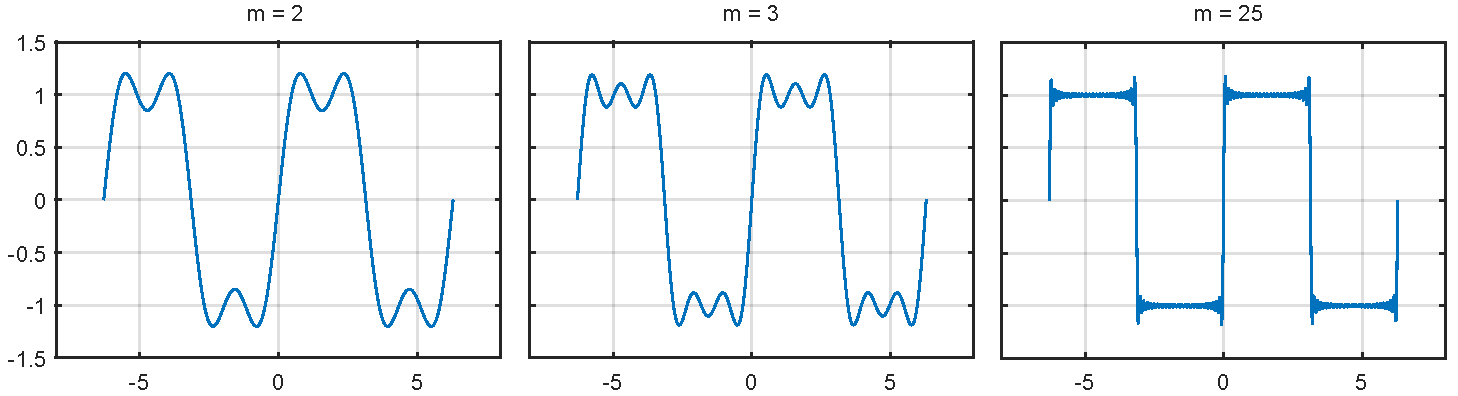
\includegraphics[width=14.25cm]{./figures/FSTri_1.pdf}
\caption{有限项傅里叶级数逼近方波}\label{FSTri_fig1}
\end{figure}
\end{example}

\begin{example}{正弦函数的绝对值} % 未完成:图

偶函数 $f(x) = \abs{\sin x}$ 存在不光滑的点,展开成傅里叶级数为
\begin{equation}\label{FSTri_eq6}
f(x) = \abs{\sin x} = \frac{2}{\pi } - \frac{4}{\pi }\sum_{k = 1}^{+\infty} \frac{1}{4 k^2 - 1}\cos 2k x
\end{equation}
前 $m$ 项和画图如\autoref{FSTri_fig2}.
\begin{figure}[ht]
\centering
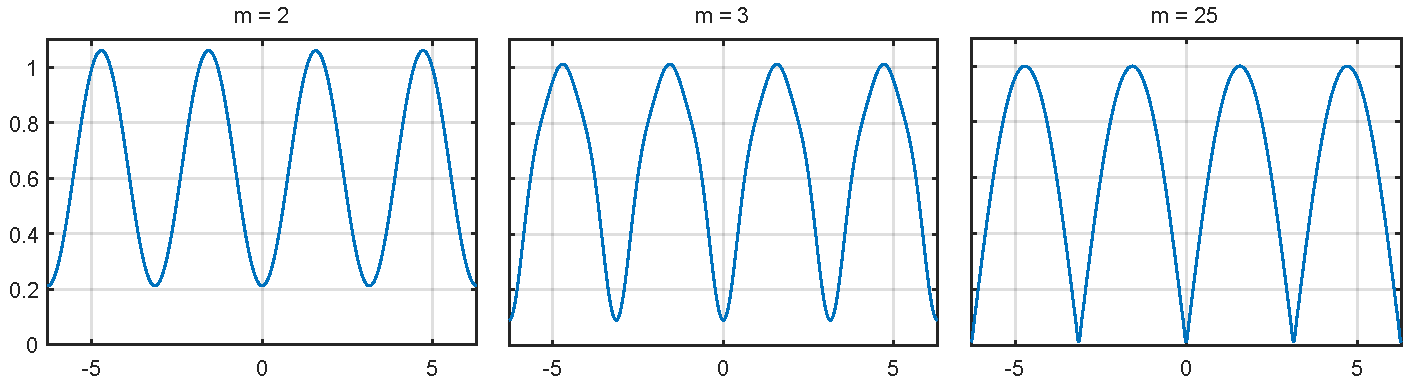
\includegraphics[width=14.25cm]{./figures/FSTri_2.pdf}
\caption{有限项傅里叶级数逼近 $\abs{\sin(x)}$}\label{FSTri_fig2}
\end{figure}
\end{example}

\begin{exercise}{}
根据傅里叶级数的定义用定积分计算\autoref{FSTri_eq5} 和\autoref{FSTri_eq6}.
\end{exercise}


\subsection{系数公式推导}
\pentry{正交归一基底\upref{OrNrB}}

在泰勒级数\upref{Taylor}中,% 链接未完成
我们通过求 $n$ 阶导数的方式来“过滤”出第 $n$ 阶系数.这里我们用积分的方式来“ 过滤” 系数.我们在推导中还要介绍一个重要的类比来讲解,即把级数中的 $\sin$ 和 $\cos$ 的性质对比几何矢量在正交(不归一)基底上的展开(\autoref{OrNrB_eq1}~\upref{OrNrB}).

% 感觉先上图最容易懂. 还是先说 sin&cos 基底再介绍单独的 sin 基底 (注意包括 “1”)(cos 基底提一下就好), 用于某个区间内的函数,不需要拓展成周期函数的情况.
% 

给出一组无穷多个函数
\begin{equation}\label{FSTri_eq4}
\begin{aligned}
&\frac12,\;   \sin(\frac{\pi}{l} x),\;   \cos(\frac{\pi}{l} x),\;   \sin(\frac{2\pi}{l} x),\;   \cos(\frac{2\pi}{l} x),\;   \dots\\
&\sin(\frac{n\pi}{l} x),\;   \cos(\frac{n\pi}{l} x)\;   \dots
\end{aligned}\end{equation}
其中 $n$ 是正整数.我们把任意满足狄利克雷条件的函数(以下简称任意函数)比作几何矢量,把上面这组函数(\autoref{FSTri_eq4})比作矢量基底(称为\textbf{函数基底})
,任意函数都可以表示成这组基底的线性组合(即\autoref{FSTri_eq1}).现在把两个任意函数(矢量) $f(x)$ 和 $g(x)$ 的\textbf{内积}定义为它们的乘积在 $[-l,l]$ 内积分
\begin{equation}
\braket{f}{g} = \int_{-l}^{l} f(x)g(x) \dd{x}
\end{equation}
可以证明这组基底\textbf{正交}(即任意两个不同的基底内积为 0,证明见下文)但不\textbf{归一}\footnote{归一化的矢量也叫单位矢量, 与自身内积等于 1, 详见 “矢量内积”\upref{Dot}}.与 “几何矢量在正交但不归一的基底上展开” 一样,我们只要把函数分别与各个基底内积,再除以基底的模长平方(模方)
即可获得线性组合的系数 $a_n$ 和 $b_n$. 可以证明所有基底的模方为 $l$, 这样我们就得到了系数公式(\autoref{FSTri_eq2} \autoref{FSTri_eq3}).


\subsection{正弦基底}
若我们只需要在一个区间 $[0,l]$ 上展开函数 $f(x)$ 而不在意其他地方,那么我们可以假想 $f(x)$ 是以 $2l$ 为周期的奇函数,这样,我们只需要用正弦基底展开 $f(x)$ 即可\footnote{显然我们也可以假想 $f(x)$ 是以 $2l$ 为周期的偶函数,用余弦基底展开 $f(x)$.选择正弦或余弦还应该考虑到函数在该区间的边界条件: 正弦可以保证两端函数值为 0, 余弦可以保证区间的导数值为 0.}. 于是我们可以说,\autoref{FSTri_eq4} 中给出的所有正弦基底在区间 $[0,l]$ 具有完备性.

\begin{example}{用正弦基底展开闭区间内的函数}

\begin{figure}[ht]
\centering
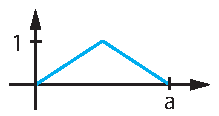
\includegraphics[width=4cm]{./figures/FSTri_3.pdf}
\caption{三角形函数} \label{FSTri_fig3}
\end{figure}

定义区间 $[0,a]$ 内的一个三角形函数如下(\autoref{FSTri_fig3}),先把函数归一化,再用正弦基底做傅里叶展开.
\begin{equation}
f(x) = \leftgroup{
&\frac2a x &\quad \qty(0 \leqslant x \leqslant \frac a2)\\
&2 -\frac2a x &\quad \qty(\frac a2 < x \leqslant a)
}\end{equation}

首先假想 $f(x)$ 为奇函数,原则上可以直接使用\autoref{FSTri_eq3} 计算展开系数,但由于被积函数 $f(x)\sin(x)$ 为偶函数, 可以先把\autoref{FSTri_eq3} 化简为%未完成:介绍定积分的时候也讲讲偶函数奇函数的化简呗
\begin{equation}
{b_n} = \frac{2}{a}\int_{0}^a f( x )\sin (\frac{n\pi}{a}x) \dd{x}
\end{equation}

又注意 $f(x)$ 关于区间中点的对称性,我们可以进一步判断出 $n$ 为偶数时 $b_n$ 项都为零, 而 $n$ 为奇数项的 $b_n$ 在 $[0, a/2]$ 的积分等于在 $[a/2, a]$ 的积分, 所以
\begin{equation}
\ali{
{b_n} &= \frac{4}{a}\int_{0}^{a/2} f( x )\sin (\frac{n\pi}{a}x) \dd{x}\\
&= \frac{8}{a^2} \int_{0}^{a/2} x\sin (\frac{n\pi}{a}x) \dd{x}
}\end{equation}
这个积分既可以见例*%未完成:例子放到分部积分里面吧
,也可以用 Wolfram Alpha 或 Mathematica 完成.%未完成:链接
结果是
\begin{equation}
b_n = (-1)^{\frac{n-1}{2}} \frac{8}{\pi^2 n^2} \quad (\text{$n$ 为奇数})
\end{equation}

\end{example}

进一步说,我们可以用正弦基底在任意区间 $[x_0,x_0+l]$ 上展开任意函数.要这样做,我们只需要把所有正弦基底平移 $x_0$ 即可.
\begin{equation}
\sin\frac{\pi}{l} (x-x_0),\;   \sin\frac{2\pi}{l} (x-x_0),\;    \dots\;\sin\frac{n\pi}{l} (x-x_0) \dots
\end{equation}

\subsection{证明函数基底正交}

现在证明\autoref{FSTri_eq4} 中任意两个不同的基底内积等于 0.当 $m \ne n$ 时,有
\begin{equation}\ali{
&\int_{ - \pi }^\pi  \sin(mx) \sin(nx) \dd{x} \\
 = &\frac12 \int_{-\pi}^\pi  \cos [(m - n)x] \dd{x}  - \frac12\int_{-\pi}^\pi  \cos [(m + n)x] \dd{x}  = 0
}\end{equation}

\begin{equation}\ali{
&\int_{-\pi}^\pi  \cos(mx) \cos(nx) \dd{x} \\
 =  &-\frac12 \int_{-\pi}^\pi  \cos[(m - n)x] \dd{x}  + \frac12 \int_{-\pi}^\pi  \cos [(m + n)x] \dd{x}  = 0
}\end{equation}

\begin{equation}\ali{
&\int_{-\pi}^\pi  \sin(mx)  \cos(nx) \dd{x}\\
= &\frac12 \int_{-\pi}^\pi  \sin[(m + n)x] \dd{x}  - \frac12 \int_{-\pi}^\pi  \sin [(m - n)x] \dd{x} = 0
}\end{equation}

\begin{equation}
\int_{-\pi}^\pi  1 \cdot \sin x \dd{x}  = 0
\end{equation}

\begin{equation}
\int_{-\pi}^\pi  1 \cdot \cos x \dd{x}  = 0\\
\end{equation}
其中任意一个函数与自己内积都等于 $\pi $(除了常函数1积分为 $2\pi$).
\begin{equation}
\int_{-\pi}^\pi \sin[2](nx) \dd{x} = \pi
\end{equation}
\begin{equation}
\int_{-\pi}^\pi \cos[2](nx) \dd{x} = \pi
\end{equation}
\begin{equation}
\int_{-\pi}^\pi 1^2 \dd{x} = 2\pi
\end{equation}

\subsection{使用归一化的基底}

我们也可以将\autoref{FSTri_eq4} 的每个基底乘以一个常数进行归一化, 即让每个基底的模长为 1. 我们将归一化后的正弦项和余弦项分别记为 $\ket{S_n}$, $\ket{C_n}$ ($n = 1, 2,\dots$), 将常数项记为 $\ket{C_0}$.
\begin{equation}
\braket{S_n}{S_n} = \int_{-l}^l \qty[B_n \sin(\frac{n\pi}{l}x)]^2 \dd{x} = 1
\end{equation}
\begin{equation}
\braket{C_n}{C_n} = \int_{-l}^l \qty[A_n \cos(\frac{n\pi}{l}x)]^2 \dd{x} = 1
\end{equation}
解得 $A_n = B_n = 1/\sqrt{l\ }$. 最后将常数项归一化变为 $1/\sqrt{2l}$ 即可. 所以正交归一得傅里叶级数基底为
\begin{equation}
\frac{1}{\sqrt{2l}},\;   \frac{1}{\sqrt{l\ }}\sin(\frac{\pi}{l} x),\;   \frac{1}{\sqrt{l\ }}\cos(\frac{\pi}{l} x),\;   \dots\;  \frac{1}{\sqrt{l\ }}\sin(\frac{n\pi}{l} x),\;   \frac{1}{\sqrt{l\ }}\cos(\frac{n\pi}{l} x)\;   \dots
\end{equation}
易证将基底乘以常数不影响它们的正交性, 我们可以将正交归一基底的性质用克罗内克 $\delta$ 函数(\autoref{OrNrB_eq2}~\upref{OrNrB})表示(常数基底可以记为 $\ket{C_0}$)
\begin{equation}
\braket{S_m}{S_n} = \delta_{m,n}
\qquad
\braket{C_m}{C_n} = \delta_{m, n}
\qquad
\braket{S_m}{C_n} = 0
\end{equation}

如果将任意函数 $f(x)$ 记为 $\ket{f}$, 傅里叶级数的公式可以记为(下面默认 $\ket{C_n}$ 求和时 $n = 0, 1, \dots$, 对 $\ket{S_n}$ 求和时 $n = 1, 2, \dots$)
\begin{equation}
\ket{f} = \sum_n \qty(a_n \ket{C_n} + b_n \ket{S_n})
\end{equation}
\begin{equation}
a_n = \braket{f}{C_n}
\qquad
b_n = \braket{f}{S_n}
\end{equation}
这比上文的定义要更简洁. 我们还可以证明两函数 $f(x)$ 和 $g(x)$ 的内积为
\begin{equation}
\begin{aligned}
\braket{f}{g} &= \sum_m \qty(a_m \bra{C_m} + b_m \bra{S_m}) \sum_n \qty(c_n \ket{C_n} + d_n \ket{S_n})\\
&= \sum_{m, n} a_m c_n \delta_{m, n} + b_m d_n \delta_{m, n}\\
&= \sum_n (a_n c_n + b_n d_n)
\end{aligned}
\end{equation}
该式可以类比几何矢量的坐标计算(\autoref{Dot_eq4}~\upref{Dot}), 即把两个函数在所有基底上的展开系数分别相乘再相加.

特殊地, 一个任意函数的模方为
\begin{equation}
\braket{f} = \sum_n (a_n^2 + b_n^2)
\end{equation}
即将所有展开系数分别平方再相加. 这与几何矢量模方公式也相同.

